\documentclass[aspectratio=169,11pt]{beamer}

\usetheme{Madrid}
\usecolortheme{dolphin}
\setbeamertemplate{navigation symbols}{}
\setbeamertemplate{footline}[frame number]

\usepackage{amsmath,amssymb}
\usepackage{booktabs}
\usepackage{listings}
\usepackage{xcolor}
\usepackage{tikz}
\usetikzlibrary{arrows.meta,positioning}

\definecolor{leanblue}{RGB}{38,90,150}
\definecolor{solverorange}{RGB}{213,112,39}
\definecolor{proofgreen}{RGB}{45,130,90}
\definecolor{softgray}{RGB}{245,247,250}

\setbeamercolor{structure}{fg=leanblue}
\setbeamercolor{block title}{bg=leanblue!15,fg=black}
\setbeamercolor{block body}{bg=softgray,fg=black}
\setbeamercolor{alerted text}{fg=solverorange!85!black}

\lstset{
  basicstyle=\ttfamily\scriptsize,
  columns=fullflexible,
  keepspaces=true,
  showstringspaces=false,
  frame=single,
  framerule=0.3pt,
  rulecolor=\color{black!25},
  backgroundcolor=\color{softgray},
  breaklines=true
}

\newcommand{\vipr}{\textsc{VIPR}}
\newcommand{\scip}{\textsc{SCIP}}
\newcommand{\lean}{\textsc{Lean 4}}
\newcommand{\code}[1]{\texttt{#1}}

\title{VIPR (\emph{Verifying Integer Programming Results})\\
Proof Certificates and a Kernel-Checked Lean Verifier}
\author{}
\date{September 2026}

\begin{document}

\begin{frame}
  \titlepage
\end{frame}

\begin{frame}{Mixed-integer linear programming (MILP)}
  Split the decision variables into continuous values
  $x\in\mathbb{R}^{n}$ and integer decisions $z\in\mathbb{Z}^{p}$:
  \[
    \min_{x,z}\; c_x^\mathsf{T}x+c_z^\mathsf{T}z
    \qquad\text{subject to}\qquad
    A_xx+A_zz\leq b.
  \]

  \begin{columns}[T]
    \begin{column}{0.47\textwidth}
      \begin{block}{What the symbols mean}
        \begin{itemize}
          \item $x$: continuous quantities, including fractional values
          \item $z$: integer variables, often binary choices
          \item $A_x,A_z,b$: linear constraints
          \item $c_x,c_z$: objective coefficients
        \end{itemize}
      \end{block}
    \end{column}
    \begin{column}{0.49\textwidth}
      \begin{block}{LP, ILP, and MILP}
        \begin{itemize}
          \item Linear programming (LP): only continuous variables
          \item Integer linear programming (ILP): only integer variables
          \item Mixed-integer linear programming (MILP): both kinds appear
        \end{itemize}
      \end{block}
    \end{column}
  \end{columns}
\end{frame}

\begin{frame}{Neural-network example: one rectified linear unit (ReLU)}
  Consider
  \[
    0\leq u\leq0.6,\qquad t=2u-1,\qquad v=\max(t,0).
  \]
  Use continuous variables $u,t,v\in\mathbb{R}$ and one binary variable
  $a\in\{0,1\}$ indicating whether the ReLU is active:
  \[
    v\geq0,\qquad v\geq t,\qquad
    v\leq t+1-a,\qquad v\leq0.2a.
  \]

  \begin{columns}[T]
    \begin{column}{0.47\textwidth}
      \begin{block}{Meaning of the binary variable}
        \begin{itemize}
          \item $a=0$ forces $v=0$ and $t\leq0$
          \item $a=1$ forces $v=t$ and $t\geq0$
        \end{itemize}
        Thus the linear constraints encode $v=\max(t,0)$ exactly.
      \end{block}
    \end{column}
    \begin{column}{0.49\textwidth}
      \begin{block}{Turn safety into infeasibility}
        To prove $v<0.3$ for every allowed input, add the unsafe condition
        \[
          v\geq0.3.
        \]
        A feasible solution is a concrete counterexample. If the MILP is infeasible,
        no such input exists.
      \end{block}
    \end{column}
  \end{columns}
\end{frame}

\begin{frame}{Why use proof certificates?}
  \begin{columns}[T]
    \begin{column}{0.55\textwidth}
      \begin{itemize}
        \item Mixed-integer programming (MIP) solvers are large systems containing
              branch-and-bound, cutting planes, linear-programming (LP) algorithms,
              presolving, and heuristics.
        \item A wrong ``infeasible'' answer can invalidate the final safety claim.
        \item A certificate records a derivation that can be checked without
              repeating the expensive search.
        \item This separates \emph{finding} a proof from \emph{validating} it.
      \end{itemize}
    \end{column}
    \begin{column}{0.41\textwidth}
      \begin{block}{Certificate approach}
        Let the solver perform the expensive search, but require it to emit a
        small, independently checkable proof.
      \end{block}
      \vspace{0.5em}
      \begin{alertblock}{Remaining problem}
        If the certificate checker is unverified, the checker itself becomes
        part of the trusted computing base.
      \end{alertblock}
    \end{column}
  \end{columns}
\end{frame}

\begin{frame}{Analogy with Boolean satisfiability (SAT)}
  \footnotesize
  \begin{tabular}{@{}p{0.27\textwidth}p{0.30\textwidth}p{0.34\textwidth}@{}}
    \toprule
    & Boolean SAT & Mixed-integer programming (MIP) \\
    \midrule
    Candidate model &
      Boolean assignment &
      Continuous/integer variable assignment \\[0.5em]
    Successful model &
      All clauses are satisfied &
      All linear and integrality constraints are satisfied \\[0.5em]
    No model exists &
      Formula is \alert{unsatisfiable (UNSAT)} &
      MIP is \alert{infeasible} \\[0.5em]
    Proof certificate &
      DRAT/LRAT clause-proof derivation &
      \vipr{} constraint derivation \\[0.5em]
    Final contradiction &
      Empty clause $\bot$ &
      Absurd row such as $0\leq -1$ \\
    \bottomrule
  \end{tabular}

  \vspace{0.8em}
  \begin{block}{Same proof-producing architecture}
    The solver performs the search and emits a certificate. A much smaller checker
    validates each derivation step and confirms that the proof ends in contradiction.
  \end{block}

  \vspace{0.3em}
  SAT certificates derive clauses; \vipr{} certificates derive exact linear
  constraints and additionally justify rounding and integer case splits.
\end{frame}

\begin{frame}[fragile]{How the problem and proof appear in VIPR}
  \begin{columns}[T]
    \begin{column}{0.43\textwidth}
      \begin{description}
        \item[\code{VER}] format version
        \item[\code{VAR}] variable names and indices
        \item[\code{INT}] integer-constrained variables
        \item[\code{OBJ}] objective linear form
        \item[\code{CON}] original constraint rows
        \item[\code{RTP}] relation to prove
        \item[\code{SOL}] primal solutions
        \item[\code{DER}] derived constraints
      \end{description}
    \end{column}
    \begin{column}{0.53\textwidth}
\begin{lstlisting}
VER 1.0
VAR 3  y x z
INT 3  0 1 2
OBJ min 0
CON 8 6
  C0 E 23  3 0 10 1 6 2 15
  ...
RTP infeas
SOL 0
DER 32
  A9  L 0 1 0 1 { asm } -1
  A10 G 1 1 0 1 { asm } -1
  D14 L 0 1 2 1 { rnd 1 13 1 } -1
  D27 L -1 0    { lin ... } -1
  D38 L -2 0    { lin ... } -1
  D39 G 1 0   { uns 27 10 38 9 } -1
\end{lstlisting}
    \end{column}
  \end{columns}

  \vspace{0.3em}
  Constraint indices refer to the running pool: first the \code{CON} rows, then
  previously derived \code{DER} rows.
\end{frame}

\begin{frame}{The four proof rules used for infeasibility}
  \small
  \begin{tabular}{@{}p{0.11\textwidth}p{0.38\textwidth}p{0.42\textwidth}@{}}
    \toprule
    Rule & Certificate meaning & What the checker validates \\
    \midrule
    \code{asm} &
      Introduce a branch assumption. &
      Record the stated row as an open assumption. \\[0.5em]
    \code{lin} &
      Derive a row by a suitable signed rational combination. &
      Multiplier signs, exact combined form, and right-hand-side domination. \\[0.5em]
    \code{rnd} &
      Apply a linear combination and integer rounding. &
      The combination is valid and its form is integer-valued; then use
      floor or ceiling. \\[0.5em]
    \code{uns} &
      Merge two branches of an integer split. &
      The branch rows imply the result and the discharged bounds are
      complementary: $f\leq k$ or $f\geq k+1$. \\
    \bottomrule
  \end{tabular}

  \vspace{1em}
  \begin{block}{Acceptance condition for \code{RTP infeas} in the current checker}
    The last derived row must be an absurdity such as $0\leq -1$, and it must
    have no remaining open assumptions.
  \end{block}
\end{frame}

\begin{frame}[fragile]{Lean semantics: small and exact}
  \begin{columns}[T]
    \begin{column}{0.52\textwidth}
\begin{lstlisting}
abbrev Valuation := Nat -> Rat

structure SLe where
  sense : Char
  form  : LinForm
  rhs   : Rat

def SLe.sat (c : SLe) (a : Valuation) : Prop :=
  if c.sense = 'L' then c.form.eval a <= c.rhs
  else if c.sense = 'G' then c.rhs <= c.form.eval a
  else if c.sense = 'E' then c.form.eval a = c.rhs
  else False
\end{lstlisting}
    \end{column}
    \begin{column}{0.44\textwidth}
      \begin{itemize}
        \item Every coefficient and comparison uses exact
              $\mathbb{Q}$ arithmetic.
        \item Sparse forms are lists of
              \[
                (\text{variable index},\text{coefficient}).
              \]
        \item No floating-point tolerance is used during replay.
        \item The soundness proofs are stated directly against
              \code{SLe.sat}.
      \end{itemize}
    \end{column}
  \end{columns}
\end{frame}

\begin{frame}{Rule-level soundness theorems}
  \small
  \begin{description}
    \item[\code{linCheck\_sound}]
      If the referenced rows hold and the Boolean linear-combination check returns
      \code{true}, then the stated row holds.

    \item[\code{rndCheck\_sound}]
      The same conclusion after proving that the combined form is integer-valued
      and applying exact floor/ceiling rounding.

    \item[\code{unsBounds\_split}]
      Complementary integer bounds cover every valuation satisfying the declared
      integrality conditions.

    \item[\code{domSLe\_sat}]
      If a checked row dominates the stated row, satisfaction of the first implies
      satisfaction of the second.
  \end{description}

  \begin{block}{Proof style}
    Each executable predicate has a theorem of the form
    \[
      \texttt{check data = true}\quad\Longrightarrow\quad
      \text{semantic consequence}.
    \]
    The checker is reflective, but its reflection theorem is checked by the Lean kernel.
  \end{block}
\end{frame}

\begin{frame}[fragile]{Example Lean theorem: \code{rndCheck\_sound}}
\begin{lstlisting}
theorem rndCheck_sound {intVars stated cs}
    (h : rndCheck intVars stated cs = true)
    {a : Valuation}
    (hint : forall j, List.Mem j intVars ->
      IsIntVal (a j))
    (hsat : forall p, List.Mem p cs ->
      p.2.sat a) :
    stated.sat a
\end{lstlisting}

  \begin{block}{Meaning}
    If the Boolean \code{rndCheck} accepts, every referenced row is satisfied,
    and the declared variables are integer-valued, then the rounded row is
    semantically satisfied.
  \end{block}
\end{frame}

\begin{frame}[fragile]{Main soundness chain}
  \begin{center}
  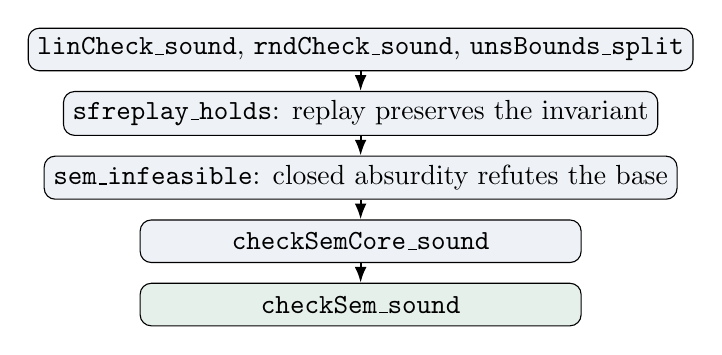
\begin{tikzpicture}[
      node distance=0.25cm,
      thm/.style={draw,rounded corners,minimum width=5.6cm,minimum height=0.54cm,
                  align=center,fill=leanblue!8},
      arr/.style={-{Latex[length=2mm]},thick}
    ]
    \node[thm] (rules) {\code{linCheck\_sound}, \code{rndCheck\_sound},
                       \code{unsBounds\_split}};
    \node[thm,below=of rules] (replay) {\code{sfreplay\_holds}: replay preserves the invariant};
    \node[thm,below=of replay] (inf) {\code{sem\_infeasible}: closed absurdity refutes the base};
    \node[thm,below=of inf] (core) {\code{checkSemCore\_sound}};
    \node[thm,below=of core,fill=proofgreen!12] (top) {\code{checkSem\_sound}};
    \draw[arr] (rules) -- (replay);
    \draw[arr] (replay) -- (inf);
    \draw[arr] (inf) -- (core);
    \draw[arr] (core) -- (top);
  \end{tikzpicture}
  \end{center}

\vspace{-0.35em}
\begin{lstlisting}
theorem checkSem_sound (v : Vipr) (h : checkSem v = true) :
  forall a,
    (forall j in v.intVars, IsIntVal (a j)) ->
    (forall c in conSLes v, SLe.sat c a) ->
    False
\end{lstlisting}

  Acceptance therefore means that the certificate's own \code{CON} system is
  infeasible over its declared integer variables.
\end{frame}

\begin{frame}[fragile]{Highlight: verified checker $\neq$ certified run}
  \begin{columns}[T]
    \begin{column}{0.47\textwidth}
      \begin{alertblock}{Compiled CLI}
\begin{lstlisting}[basicstyle=\ttfamily\scriptsize]
if checkSem cert then
  IO.println "ACCEPT"
else
  IO.println "REJECT"
\end{lstlisting}
        \footnotesize
        This returns a machine Boolean. Trusting ``ACCEPT'' also trusts the
        compiled execution of \code{checkSem}, its runtime, and the CLI path.
      \end{alertblock}
    \end{column}
    \begin{column}{0.49\textwidth}
      \begin{block}{Kernel reflection}
\begin{lstlisting}[basicstyle=\ttfamily\scriptsize]
theorem accepted :
    checkSem cert = true := by
  decide +kernel

theorem infeasible :=
  checkSem_sound cert accepted
\end{lstlisting}
        \footnotesize
        The kernel evaluates this concrete check and validates the proof term.
        The artifact generator may be untrusted: bad output fails kernel checking.
      \end{block}
    \end{column}
  \end{columns}

  \begin{block}{The crucial distinction}
    \footnotesize
    \begin{tabular}{@{}p{0.25\textwidth}@{\quad}p{0.65\textwidth}@{}}
      \textbf{Checker soundness} &
      If \code{checkSem v = true}, then the represented system is infeasible.\\[0.35em]
      \textbf{Certified run} &
      The kernel has proved \code{checkSem cert = true} for this certificate.
    \end{tabular}
  \end{block}

  \tiny
  \textbf{TCB caveat:} ``Kernel-only'' still trusts Lean's kernel; it excludes
  separately compiled checker execution and runtime from this certificate's trusted path.
\end{frame}

\begin{frame}[fragile]{Concrete certificates are checked by kernel reduction}
\begin{lstlisting}[basicstyle=\ttfamily\tiny]
theorem acceptedSlice : checkSem sliced = true := by
  decide +kernel

theorem certified :
    forall a,
      (forall j in original.intVars, IsIntVal (a j)) ->
      (forall c in conSLes original, SLe.sat c a) ->
      False :=
  checkSem_subset_sound
    original sliced sameIntVars rowsSubset acceptedSlice
\end{lstlisting}

  \begin{columns}[T]
    \begin{column}{0.48\textwidth}
      \small
      \begin{block}{Kernel replay}
        The concrete Boolean result is reduced inside the kernel; it is not accepted
        merely because compiled command-line interface (CLI) code returned
        \code{true}.
      \end{block}
    \end{column}
    \begin{column}{0.48\textwidth}
      \small
      \begin{block}{Untrusted reconstruction}
        A native slicer removes unused proof branches. The kernel separately checks:
        same integer variables, row inclusion, and validity of the sliced proof.
      \end{block}
    \end{column}
  \end{columns}

  \vspace{0.1em}
  \small
  Example: the largest benchmark slice shrinks from 983 to 281 derivation steps,
  reducing kernel replay from about 182 seconds to 40 seconds.
\end{frame}

\begin{frame}{VIPR-only benchmark: list replay and reconstruction}
  \scriptsize
  \begin{center}
  \begin{tabular}{@{}lrrrrr@{}}
    \toprule
    Certificate & KiB & steps & compiled & full list & reconstructed \\
    \midrule
    knapsack & 1.99 & $32\to23$ & 0.04 & 22.98 & 22.61 \\
    NN leaf $[-4]$ & 7.54 & $97\to13$ & 0.04 & 28.62 & 24.10 \\
    NN leaf $[-2,4]$ & 22.43 & $273\to72$ & 0.05 & 28.13 & 24.99 \\
    NN leaf $[2,1,4]$ & 16.13 & $177\to11$ & 0.04 & 25.02 & 24.71 \\
    NN leaf $[2,-1,4]$ & 82.05 & $983\to281$ & 0.07 & 181.81 & 39.67 \\
    \midrule
    \textbf{Total} & \textbf{130.14} & $\mathbf{1562\to400}$ &
      \textbf{0.24} & \textbf{286.56} & \textbf{136.08} \\
    \bottomrule
  \end{tabular}
  \end{center}

  \vspace{0.5em}
  \begin{itemize}
    \item Times are seconds on identical VIPR certificate files; steps show
          complete certificate $\to$ checked slice.
    \item The compiled CLI is an untrusted performance reference. Full list replay
          and reconstruction both produce kernel-checked theorems.
    \item Reconstruction retains the original list-backed checker and reduces total
          kernel wall time by $52.51\%$ ($2.11\times$ faster).
  \end{itemize}

  \vspace{0.2em}
  \centering
  \tiny Apple M3 Pro (12 cores, 36 GB), Lean 4.31.0; one warmed sequential run.
\end{frame}

\begin{frame}{What is trusted, and what is not?}
  \begin{columns}[T]
    \begin{column}{0.48\textwidth}
      \begin{block}{Trusted for the abstract-syntax-tree (AST) theorem}
        \begin{itemize}
          \item Lean kernel
          \item Definitions of constraint satisfaction and infeasibility
          \item Mathlib's exact rational arithmetic
          \item Three standard axioms:
                \code{propext}, \code{Classical.choice}, \code{Quot.sound}
        \end{itemize}
      \end{block}
    \end{column}
    \begin{column}{0.48\textwidth}
      \begin{alertblock}{Untrusted witness production}
        \begin{itemize}
          \item \scip{} and its search
          \item Certificate slicing
          \item Native prechecks
          \item Proof-data generation
        \end{itemize}
        Bad output should cause kernel rejection, not false certification.
      \end{alertblock}
    \end{column}
  \end{columns}

  \vspace{0.5em}
  Tactics such as \code{linarith} are not trusted: they generate proof terms that
  the kernel independently checks.
\end{frame}

\begin{frame}{Current scope and remaining frontend gap}
  \begin{itemize}
    \item The proved theorem is relative to the emitted \code{Vipr} abstract syntax
          tree (AST).
    \item The generated artifact currently embeds both \code{sourceText} and the AST,
          but does not yet prove
          \[
            \code{parseVipr sourceText = .ok original}.
          \]
    \item The parser currently ignores trailing tokens, and the semantic checker does
          not enforce \code{RTP infeas}.
    \item \code{asm}/\code{lin}/\code{rnd}/\code{uns} infeasibility replay is covered;
          objective-range and \code{sol} result semantics are not fully checked.
  \end{itemize}

  \begin{block}{Next trust-hardening step}
    Reject trailing tokens, require the infeasibility RTP, and kernel-check the
    concrete parser equation so that the theorem is bound to the exact certificate text.
  \end{block}
\end{frame}

\begin{frame}{Takeaways}
  \begin{enumerate}
    \item A proof-producing solver lets us separate expensive search from trusted
          verification.
    \item \vipr{} records a flat derivation using linear combinations, integer
          rounding, assumptions, and branch merging.
    \item The Lean checker replays these rules over exact rationals and proves a
          semantic invariant for every pool entry.
    \item \code{checkSem\_sound} reduces acceptance to a kernel-checked theorem:
          no integral valuation satisfies the certified constraints.
    \item Reconstruction improves performance without trusting the slicer, while
          parser-to-source binding remains the main frontend task.
  \end{enumerate}

  \vspace{0.8em}
  \begin{center}
    \Large
    \alert{Untrusted search} \quad+\quad
    \textcolor{proofgreen}{kernel-checked replay}
    \quad=\quad a small, auditable trust base
  \end{center}
\end{frame}

\begin{frame}{References}
  \small
  \begin{itemize}
    \item Kevin K.\ H.\ Cheung, Ambros Gleixner, and Daniel E.\ Steffy.
          \emph{Verifying Integer Programming Results}. IPCO 2017.
    \item The \vipr{} reference implementation: \code{github.com/scipopt/vipr}.
    \item Project sources:
      \begin{itemize}
        \item \code{ViprCheck/Cert/ViprSem.lean}
        \item \code{ViprCheck/Pipeline/Vipr.lean}
        \item \code{ViprMain.lean}
      \end{itemize}
  \end{itemize}
\end{frame}

\end{document}
